\title{Singularity Software\\Milestone 1}
\date{\today}

\documentclass[12pt]{article}
\usepackage[a4paper]{geometry}
\usepackage{makeidx}
\usepackage[acronym]{glossaries}
\usepackage{lscape}
\usepackage{amsmath}
% \usepackage{hyperref} % Makes links from ToC

\geometry{top=1.0in, bottom=1.0in, left=1.0in, right=1.0in} % Sets the margins

\setlength{\parindent}{0pt} % Fixes the paragraph spacing problem

% This is all for formatting and making the Table of Contents according to 
% spec. Don't play with it.
\makeatletter
\renewcommand\l@section[2]{%
  \ifnum \c@tocdepth >\z@
    \addpenalty\@secpenalty
    \addvspace{1.0em \@plus\p@}%
    \setlength\@tempdima{1.5em}%
    \begingroup
      \parindent \z@ \rightskip \@pnumwidth
      \parfillskip -\@pnumwidth
      \leavevmode \bfseries
      \advance\leftskip\@tempdima
      \hskip -\leftskip
      #1\nobreak\ 
      \leaders\hbox{$\m@th\mkern \@dotsep mu\hbox{.}\mkern \@dotsep mu$}
     \hfil \nobreak\hb@xt@\@pnumwidth{\hss #2}\par
    \endgroup
  \fi}
\makeatother

\makeindex

% Construct the glossary here
% Use the template below, then where the word appears (in the case below, computer), replace computer with \gls{computer}
\makeglossaries

\newglossaryentry{Sifteo Cubes}
{
  name={Sifteo Cubes},
  description={are small machines capable of loading programs and interacting with one another as well as responding to predefined movements}
}

\newglossaryentry{Object-Oriented Programming}
{
  name={Object-Oriented Programming},
  description={is a programming paradigm using objects to design applications}
}

\newglossaryentry{Windows}
{
  name={Windows},
  description={is a series of operating systems developed by Microsoft}
}

\newglossaryentry{Mac}
{
  name={Mac},
  description={is a series of lines of personal computers developed by Apple}
}

\newglossaryentry{Linux}
{
  name={Linux},
  description={is a Unix-based operating system based on free and open source software}
}

\newglossaryentry{cross-platform support}
{
  name={cross-platform support},
  description={is an attribute given to software implemented and operable on multiple computer platforms}
}

\newacronym{API}{API}{\glsadd{API}{Application Programming Interface}}

\newglossaryentry{APIg}
{
  name={Application Programming Interface},
  description={is an interface implemented by a software program that enables it to interact with other software}
}


\newglossaryentry{open source}
{
  name={open source},
  description={is an attribute given to software for which the source code is freely available}
}

\newacronym{IDE}{IDE}{\glsadd{IDE}{Integrated Development Environment}}

\newglossaryentry{IDEa}
{
  name={Integrated Development Environment},
  description={is software that provides a comprehensive work environment for computer programmers and software developers}
}


\newacronym{GUI}{GUI}{\glsadd{GUI}{Graphical User Interface}}

\newglossaryentry{GUIa}
{
  name={Graphical User Interface},
  description={is a visual way of allowing the user to interace with a computer program}
}

\newglossaryentry{version control}
{
  name={version control},
  description={is the management of documents and programs for a project over many versions in a well-organized manner}
}

\newglossaryentry{issue tracking system}
{
  name={issue tracking system},
  description={is a piece of software used to maintain a list of issues as generated during a project}
}

\renewcommand*\arraystretch{1.5}

\begin{document}
\vspace*{\fill}
        \begin{center}
                \LARGE{Singularity Software} \\
                \LARGE{\textit{Milestone 1}} \\
                \vspace{.15in}
                \large{\today} \\
                \vspace{4in}
                By signing below, I approve the contents of the following document. \\
                \begin{table}[h]
                        \begin{tabular}{p{2in} p{5.5in}}
%                \begin{align*}
                        & \\
                        Alex Mullans & \line(1,0){285} \\ & \\
                        Ruben Rodriguez & \line(1,0){285} \\ & \\
                        Ethan Veatch & \line(1,0){285} \\ & \\
                        Kurtis Zimmerman & \line(1,0){285}
                        \end{tabular}
                \end{table}
%                \end{align*}
        \end{center}
\vspace*{\fill}
\thispagestyle{empty}

\clearpage

\tableofcontents

\clearpage
        
\section{Executive Summary}
This document summarizes the problem addressed by the Siftables\index{Siftables} Emulator\index{emulator} project. After providing a brief summary of the clients---Tim Ekl and Eric Stokes---and the current solution, or lack thereof, it goes on to provide more detail about the stakeholders involved in the project and their primary concerns and needs. Those stakeholders include the clients and the developers of \index{Sifteo}Sifteo Cube programs, who will be the primary users of the software. Finally, an overview of the proposed product and its key requirements and features, as agreed upon by the client and Singularity Software, is detailed, and the constraints surrounding the project's development are enumerated. Future documents will use the information contained herein as a starting point from which to provide more details of the final solution.

\section{Introduction}
Developers of applications for the \gls{Sifteo Cubes}\index{Sifteo} currently must test programs they create for the platform on the Cubes themselves.  With a full release of the Cubes and corresponding \gls{API}\index{API}\glsadd{APIg} still pending, developers unable to join the Sifteo Early Access program are left without a software-based interface within which to productively develop Sifteo programs. As such, Singularity Software will provide, in the form of the Siftables Emulator, a software-based emulator\index{emulator} for the Sifteo Cubes that will allow any developer to try programming in the unqiue environment provided by the Cubes.\\\\
This document is the first in a series of milestone documents that will accompany the planning of the Siftables\index{Siftables} Emulator\index{emulator}. It will provide an overview of the current system, all involved clients and stakeholders, and a statement of the problem Singularity seeks to solve. Additionally, it will detail a list of high-level features as agreed upon with the clients. Future milestones will delve into the user cases, data flow diagrams, and prototypes necessary to convert those high-level features to a working system; as the project progresses, future milestones will also present plans for change control, coding standardization, and testing. Finally, design and usability reports will make up the core of milestones near the end of the quarter as the software stabilizes.

\section{Client Background}
Clients Tim Ekl and Eric Stokes are alumni of Rose-Hulman. Mr. Ekl is currently working on a M.S. degree in Engineering Management; Mr. Stokes is currently working for n{\raise.17ex\hbox{$\scriptstyle\sim$}}ask Signal Processing Systems in Denver, Colorado. As former Rose-Hulman students, the clients are avid users of technology who follow new trends in the industry. As a result of this interest in new technology, both Mr. Stokes and Mr. Ekl discovered and purchased Sifteo Cubes\index{Sifteo Cubes}, a revolutionary product that consists of a set of (anywhere from 1 to 6) mini computers. While both clients have a set of 3 Sifteo Cubes, they realized that not everyone interested in the project could have the luxury of physical hardware to work with. As such, they asked Singularity Software---via the Junior Project proposal process at Rose-Hulman---to construct a software emulator\index{emulator} for the Cubes that would make the development of Sifteo\index{Sifteo} applications easier, especially in the testing phase.

\section{Current System}
Currently the only system available to developers is the Siftulator, the emulator released in Sifteo's SDK.  It allows for emulation of all Cube manipulations, and the numebr of Cubes can be increased or reduced through the interface.  An API is available through the Sifteo website, and several example games have been written for use in the emulator workspace.  The Siftulator only runs on Windows machines, leaving it inaccessible to some users.  A screenshot, taken from Sifteo's developer website, is shown below.
\begin{center}
        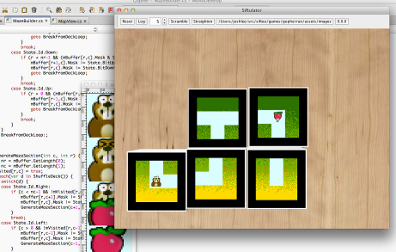
\includegraphics{siftulator.png}
\end{center}

\section{User/Stakeholder Description}

               \subsection{User/Stakeholder Profiles}

                          \subsubsection{Sifteo application developers}
                          As the primary target audience of the system, developers targeting the Sifteo\index{Sifteo} platform are assumed to have a reasonable amount of technical background; they are not novice computer users and are familiar with programming concepts like \gls{Object-Oriented Programming}\index{Object-Oriented Programming} and \gls{API}\index{API}s. As developers may hail from platforms ranging from \gls{Windows} to \gls{Mac} to \gls{Linux}, \gls{cross-platform support} is an important consideration.\\\\
                          Possible problems for this user type include an unstable or crash-prone system: as developers are writing and testing their own code, it is essential that the emulator\index{emulator} does not contribute to the failures that the user must debug. Developers will deem the emulator\index{emulator} project a success when they can successfully program and test software that uses any or all of the features of the Sifteo\index{Sifteo} cubes on their development platform.

                          \subsubsection{Clients}
                          The clients (Tim Ekl and Eric Stokes) are assumed to be a subset of the Sifteo\index{Sifteo} application developers user class. However, their programming knowledge and knowledge of the Sifteo\index{Sifteo} Cubes\index{Sifteo Cubes} is known to be more advanced than that of the average application developer. As such, their needs require that the emulator\index{emulator} is capable of being pushed to the same limits as the actual platform.

                          \subsubsection{Singularity Software}
                          Singularity Software, as the team behind Siftables\index{Siftables} Emulator\index{emulator}, is primarily interested in the creation of a finished product that can be delivered to the clients at the conclusion of the Rose-Hulman junior project cycle. As a team, we are less familiar with the Sifteo platform and are also relatively inexperienced with the scale of project the emulator\index{emulator} entails.

                          \subsubsection{Sriram Mohan (CSSE Department)}
                          As the advisor of the Junior Project, Dr. Mohan has a vested interest in the creation of a finished, deliverable product. His key responsibility is to review documents created within the scope of the Junior Project series of courses.

               \subsection{User Environments}

                          \subsubsection{Sifteo application developers}
                          The typical Sifteo application developer may be working on his own, or he may be working with a team of developers; he or they will be working on workstations or powerful development laptops that have a significant amount of graphics horsepower. They may or may not be connected to the Internet during development, depending on the location in which they are developing. Additionally, they may be \gls{Windows}, \gls{Mac}, or \gls{Linux} users and will be using various \glspl{IDE}\glsadd{IDEa} specific to their platform; integration between such \glspl{IDE} and the Siftables\index{Siftables} Emulator\index{emulator}, while possibly desirable, is not a requirement.

                          \subsubsection{Clients}
			  Mr. Stokes and Mr. Ekl are both primarily \gls{Mac} users, although both clients also own and occasionally use \gls{Windows} machines as well. Their environment is essentially the same as that of the typical Sifteo\index{Sifteo} application developer.

               \subsection{Key Needs}

                          \subsubsection{Emulate Sifteo Cubes in a desktop GUI application}
                          No emulator currently exists for the Sifteo\index{Sifteo} platform; the need is currently either filled by homebrew efforts like Mr. Ekl's Java-based emulator\index{emulator}, or circumvented by using the Cubes themselves as a testing platform. The clients envision a solution where all of the interactions possible with a set of Early Access Sifteo Cubes can be replicated in a software emulator\index{emulator}.

                          \subsubsection{Develop an API for creating applications in the emulator’s Cubes}
                          An \gls{API}\index{API} is necessary to facilitate interaction with the virtual Sifteo Cubes. Currently, no \gls{API} has been made available by Sifteo for the physical cubes, and no emulator\index{emulator} \gls{API}\index{API} exists because no emulator\index{emulator} exists. The clients would like an \gls{API}\index{API} with which the virtual Cubes can be programmed. Mr. Ekl stipulated that shadowing the official Sifteo \gls{API}\index{API}, while potentially beneficial for long-term development, is not a requirement.

                          \subsubsection{Showcase Cube/emulator functionalities with samples}
                          Sifteo currently provides example games that run on the Cubes as a showcase of what the platform can achieve and what unique features it can offer to the user. The clients would like to have a similar showcase available for the emulator as an aid in understanding both the emulator platform and the larger Sifteo Cubes\index{Sifteo Cubes} programming platform.

              \subsection{Alternatives \& Competition}
              Singularity Software's Siftables Emulator\index{emulator} will be the first software of its kind for the Cubes. The only true competition is the Sifteo Cubes themselves. The Cubes have the advantage of physicality---as tactile objects, they will always be superior in terms of user experience when compared to an emulator. However, they are expensive and only manufactured in limited quantities at the moment; the Siftables Emulator\index{emulator} is, by contrast, infinitely available as an \gls{open source}\index{open source} piece of software.

\section{Product Overview}

              \subsection{Product Perspective}
              Siftables Emulator\index{emulator} is a free independent system used to emulate the way Sifteo Cubes handle motions and interactions.

              \subsection{Elevator Statement}
              Due to the limited availability of Sifteo Cubes, developers unable to obtain a set of Cubes have no good way to test the programs they create for the platform. At Singularity Software, our goal is to develop an emulator\index{emulator} for the Cubes that will be able to emulate an arbitrary number of Sifteo Cubes\index{Sifteo Cubes} and the way they handle physical motions and interactions. Along with the emulator itself, Singularity will develop an \gls{API}\index{API} and example games and programs.
\clearpage
              \subsection{Summary of Capabilities}
              The main features of our emulator\index{emulator} work together to allow developers to quickly start Sifteo application development by making a virtual edition of the Cubes available for emulation and testing.
              \begin{table}[h]
                \begin{tabular}{p{3in} | p{3in}}
                  \textbf{Feature} & \textbf{Benefit} \\ \hline
                  Workspace where multiple cubes can be emulated
                            & A user-friendly way to develop for multiple cubes \\ \hline
                  Buttons and gestures to control the cubes
                            & An easier way to control the basic movements of the cubes in place of physical manipulations \\ \hline
                  Ability to load programs into the cubes
                            & Allows the user to test his own programs and example programs in the emulator \\ \hline
                  Example games (requirement)
                            & Gets new emulator\index{emulator} users started with the platform \\ \hline
                  \Gls{open source}\index{open source}  (requirement)
                            & Allows the community to contribute improvements to the emulator\index{emulator} \\ \hline
                  \gls{API}\index{API} (requirement)
                            & A standard way of interacting with the virtual Cubes
                \end{tabular}
              \end{table}

              \subsection{Assumptions and Dependencies}
              Sifteo\index{Sifteo} has plans to release an \gls{API}\index{API} of their own for the Cubes; Singularity will attempt to make our \gls{API}\index{API} shadow much of the language and functionality of the official Sifteo \gls{API}\index{API}. 

              \subsection{Estimate of Cost}
			  Because it is an \gls{open source} piece of software, Singularity Software does not believe that the Siftables Emulator\index{emulator} will incur any monetary costs throughout the project.
\clearpage

\section{Features}
Six attributes accompany each feature described below: 
    \begin{description}
        \item[Status:] a  measure of the feature's progress duing the project definition period, either \textit{Proposed} or \textit{Approved}
        \item[Priority:] the relative importance of each feature, either \textit{Useful}, \textit{Important}, or \textit{Critical}
        \item[Risk:] the probability that the feature will bring about undesirable events, either \textit{Low}, \textit{Medium}, or \textit{High}
        \item[Stability:] the probability that the feature will change, either \textit{Low}, \textit{Medium}, or \textit{High}
        \item[Reason:] the source of the required feature
        \item[Effort:] an estimate of the relative amount of work required to complete the feature, either \textit{Low}, \textit{Medium}, or \textit{High}
    \end{description}
    The features are outlined in the table on the following page.
    \begin{landscape}
    \begin{table}[h]
      \begin{tabular}{p{1.5in} | p{1.75in} | p{.75in} | p{.75in} | p{.75in} | p{.75in} | p{1.75in} | p{.6in}}
        \textbf{Feature} &
        \textbf{Description} &
        \textbf{Status} &
        \textbf{Priority} &
        \textbf{Risk} &
        \textbf{Stability} &
        \textbf{Reason} &
        \textbf{Effort} \\ \hline

        Individual, virtual Sifteo Cube &
        A virtual representation of a single Sifteo cube &
        Approved &
        Critical &
        Low &
        High &
        Replicates physical Sifteo Cube &
        Medium \\ \hline

        Buttons to manipulate each virtual Cube &
        Buttons on the virtual Cube will allow the user to flip and tilt it &
        Approved &
        Critical &
        Medium &
        High &
        Replaces physical actions where said actions would be impractical with a mouse &
        Medium \\ \hline

        Workspace where multiple cubes can be emulated &
        Multiple cubes will be displayed on a workspace that replicates the free-form nature of physical Sifteo Cubes\index{Sifteo Cubes} &
        Approved &
        Critical &
        Low &
        High &
        Replicates multiple Sifteo Cubes\index{Sifteo Cubes} in a natural, free-form environment &
        High \\ \hline

        Interactions between Cubes &
        The Cubes present on the workspace will communicate when they are neighbored &
        Approved &
        Critical &
        Low &
        High &
        Cubes can simulate the interactions possible with physical Cubes &
        High \\ \hline

        Load programs into the Cubes &
        The user will load his own and example programs into the emulator’s\index{emulator} Cubes &
        Approved &
        Critical &
        Medium &
        High &
        The ability to program programs for the emulator\index{emulator} is dependent on a common interface &
        High \\ \hline

        Snap Cubes to invisible grid &
        The Cubes will snap into an invisible grid when a button is clicked &
        Proposed &
        Useful &
        Medium &
        High &
        Increases productivity by allowing a quick reset if the Cubes are in disarray &
        Low \\ \hline

        Zoom Workspace &
        The Workspace will zoom to the level of an individual Cube or the whole space &
        Proposed &
        Useful &
        Low &
        High &
        Inspecting individual Cubes allows for precise checks of program \glspl{GUI}\index{GUI}\glsadd{GUIa} &
        Low \\ \hline

      \end{tabular}
    \end{table}
    \end{landscape}

\section{Constraints}
        While much of this project is open-ended, there are a few basic constraints. At the direction of the clients, all code should be \gls{open source}\index{open source} and version-controlled\glsadd{version control}. Mr. Ekl requested that the emulator run easily on \gls{Mac} as well as \gls{Windows}, with the stipulation that \gls{Linux} compatibility would satisfy the \gls{Mac} requirement for Singularity's testing purposes. In addition, the clients requested that an \gls{issue tracking system} be put in place and used throughout the development process. Finally, the emulator\index{emulator} must be completed by May 18th---the end of Spring Quarter 10th week---to satisfy the requirements of the clients and of Dr. Mohan.

\clearpage
\addcontentsline{toc}{section}{Glossary}
\printglossaries
\clearpage

\addcontentsline{toc}{section}{References}
\section*{References}

        \begin{enumerate}
                \item{Sifteo Inc. Online: http://www.sifteo.com}
                \item{Tim Ekl.  Client Meeting.  12 September 2011 12:45 p.m.}
        \end{enumerate}

\clearpage

\addcontentsline{toc}{section}{Index}
\printindex

\end{document}
